\documentclass{siproblemset}

\usepackage{multicol}
\usepackage{xcolor}

% SI Session Information
\course{MTH 1321}
\sessionnum{6}
\sessiondate{2/12/21}

\warmup{Concept Review}
\topic{The Intermediate Value Theorem}
\cooldown{Challenge Problems}

% Worksheet Information
\title{The Intermediate Value Theorem\linebreak \& Definition of the Derivative}
\sections{Section 2.8-3.2a}
\withnamespace

\begin{document}
    \maketitle
    
    \activity{Warmup}{Concept Review and Overview}{Try these problems \textbf{alone} as your peers join the session. Do your best to not refer to your notes.}{15 minutes}
    \frq{What is the Intermediate Value Theorem?}
    \smallsp
    
    \frq{What are the limit definitions of the derivative of $f(x)$ at $x=a$?}
    \smallsp
    
    \frq{What are the limit definitions of the derivative of $f(x)$?}
    \smallsp
    
    \frq{What must be true for a function $f$ to be differentiable at $x=a$?}
    \smallsp
    
    \frq{What does $f'(x)$ represent both numerically and graphically?}
    \smallsp

    \pagebreak
    
    \activity{Activity 1}{Intermediate Value Theorem}{Work together in your \textbf{breakout rooms} to answer these questions. Do your best to not refer to your notes while working on these problems.}{30 minutes}
    \frq{Determine if $25-8x^2-x^3=0$ has a solution on $[-2,4]$}
    \hugesp
    \frq{Given $g(x)=\dfrac{1}{x}$, is there some $c$ such that $g(c)=\dfrac34$ where $1\leq c\leq 2$?}
    \pagebreak
    
    \activity{Activity 2}{Limit Definition of the Derivative}{Work together in your \textbf{breakout rooms} to answer these questions. Do your best to not refer to your notes while working on these problems.}{30 minutes}
    
    \begin{multipartquestion}
        Determine both $f'(2)$ and $f'(x)$, using a limit definition for each:
        \frq{$f(x)=x^3-3x^2$}
        \Largesp
        \frq{$f(x)=\sqrt{x^2+3}$}
        \Largesp
        %        \pagebreak
        %        \frq{$f(x)=\dfrac{1}{3x-2}$}
        %        \Hugesp
        %        \frq{$f(x)=x+x^{-1}$}
    \end{multipartquestion}
    \pagebreak
    
    \activity{Cooldown}{Tangent Lines}{Try these problems \textbf{alone}. Do your best to not refer to your notes.}{30 minutes}
    
    \begin{multipartquestion}
        Use the graph below to answer the following questions.
        
        \makebox[\width][c]{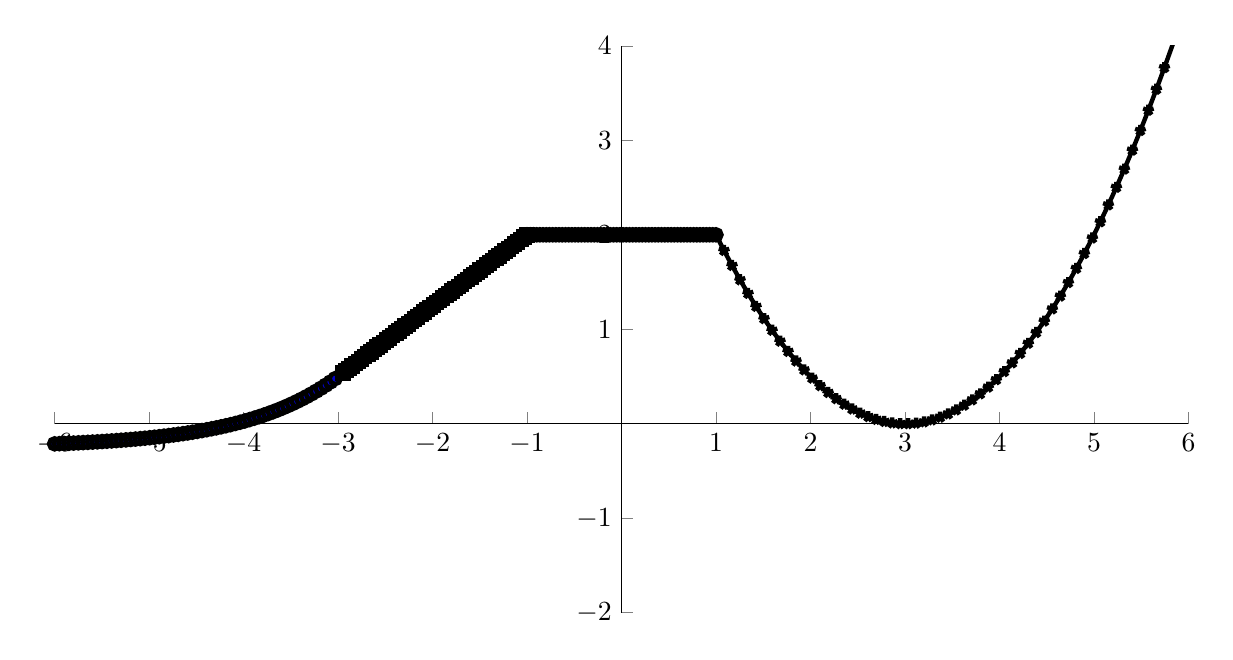
\begin{tikzpicture}[baseline=(current bounding box.north)]
            \begin{axis}[
            x=1.2cm,
            y=1.2cm,
            xmin=-6,
            xmax=6,
            ymin=-2,
            ymax=4,
            axis x line*=middle,
            axis y line*=middle,
            every axis plot/.append style={ultra thick},
            samples=60
            ]
            \addplot+[black, domain=-6:-3.03, restrict y to domain=-10:10] {e^(x+3+ln(3/4))-3/4+0.5};
            \addplot+[black, domain=-2.95:-1] {3/4*x+3/4+2};
            \addplot+[black, domain=-1:1] {2};
            \addplot+[black, domain=1:6] {1/2*(x-3)^2};
            \node at (-3,0.5) {$\circ$};
            \node at (-1,2) {\textbullet};
            \node at (1,2) {\textbullet};
            \end{axis}
            \end{tikzpicture}}
        \frq{Determine $f'(a)$ for $a=-3,-2,-1,0,1,3$. If $f$ is not differentiable at $x=a$, then state so explicitly.}
        \mediumspace
        \frq{Which is larger, $f'(2)$ or $f'(4)$? Justify your answer.}
        \nospace
        \frq{Which is larger, $|f'(2)|$ or $|f'(4)|$? Justify your answer.}
    \end{multipartquestion}
    \pagebreak
    
\end{document}